\section{Distributed databases}

\subsection{Distributed, decentralized and centralized databases}

\iffalse
- to fully comprehend distributed databases, we have to distinguish them from decentralized and centralized databases. baran 1964: in context of networks: distributed vs centralized and decentralized in between
- apply this definition to databases: add examples: one single database: standard example, decentralized: cloudfront CDN by amazon, distributed: bittorrent
\fi

To understand distributed databases, it is important to distinguish them from decentralized and centralized databases. Baran (1964) \cite{baran-distributed-communications} explains the difference in the context of networks. A centralized network makes all nodes connect to one central node. A distributed network is the opposite, in which any node can communicate with any other node without the need for a central node. Between lies the decentralized network, in which there are a couple of central nodes that communicate with each other. Other nodes have to connect with one of these central nodes.
Figure \ref{fig:baran-networks} visualizes the differences.

\begin{figure}[h]
\centering
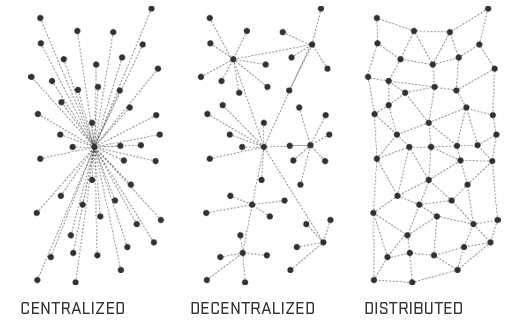
\includegraphics[width=0.8\textwidth]{paper-images/baran_networks.png}
\caption{Baran, P. (1964) Centralized, decentralized and distributed networks.} 
\label{fig:baran-networks}
\end{figure} 

This definition can be ported to the context of databases. A centralized database consists of one main data storage node. Users connect to this node to read and write data. A self-hosted website is a perfect example of a centralized database. Any user that wants to connect to your website, has to connect to your server. If your server breaks down, nobody can access the website anymore.

A decentralized database has many storage nodes that communicate with each other. A user can connect to either of these main nodes to access the data. Use of a CDN (Content Delivery Network) is an example of a decentralized database. Websites hosted on a CDN are copied across servers all over the world. To access to this website, a user can connect to any of these servers.

Finally, a distributed database does not have main storage nodes. Instead, every node can hold the entire database. When a new node wants to access the data, the node asks its peers for the data. Examples are BitTorrent and git, which both will be discussed further one in this chapter.

It is clear a trade-off is made when deciding between a centralized or distributed database. 

\iffalse
centralized => it could be that the central node is down. However, if gets repsones => for sure correct

distributed => one way or another, a new node will always be able to get an answer from the entire network.
\fi

While a user connecting to a centralized database will be sure the response is correct, 

\subsection{Consistency, availability and partition-tolerance: the CAP theorem for distributed systems}



\subsection{Advantages of using a blockchain as a distributed database}
\iffalse
- CAP Theorem
 => maybe add a section about database properties in general (CAP theorm) and the blockchain aspect of it (one of the papers mentions this, I think Bitfury)
- general advantages of blockchains as a database: consistency and consensus 
- disadvantages of blockchains: latency and scalability
\fi

\subsection{Examples of distributed databases and networks}

% how does every example do on the CAP theorm, what are other disadvantages

\subsubsection{Git}

% no authority, consensus not automatic => danger for malicious agents

\subsubsection{BitTorrent}

% no update to data

\subsubsection{Non-persistent P2P networks}

\iffalse
- no cap applicable, as not a database
- examples: open bazaar.
\fi

